\chapter{Cơ sở lý thuyết}

\section{Mạng neural}

\subsection{Mạng neural}
	
	
	Theo khái niệm về sinh học, mạng neural là sự kết nối giữa các tế bào thần kinh neural lại với nhau. Trong lĩnh vực trí tuệ nhân tạo, mạng neural còn được gọi là Artificial Neural Network (ANN) - mạng neural nhân tạo, đây là mô hình xử lý dữ liệu, mô phỏng lại chức và cách hoạt động của hệ thống neural sinh học ở con người. Hình \ref{fig:neuron} minh họa cấu trúc của tế bào thần kinh neuron.
	
	\begin{figure}[h!]
		\centering
		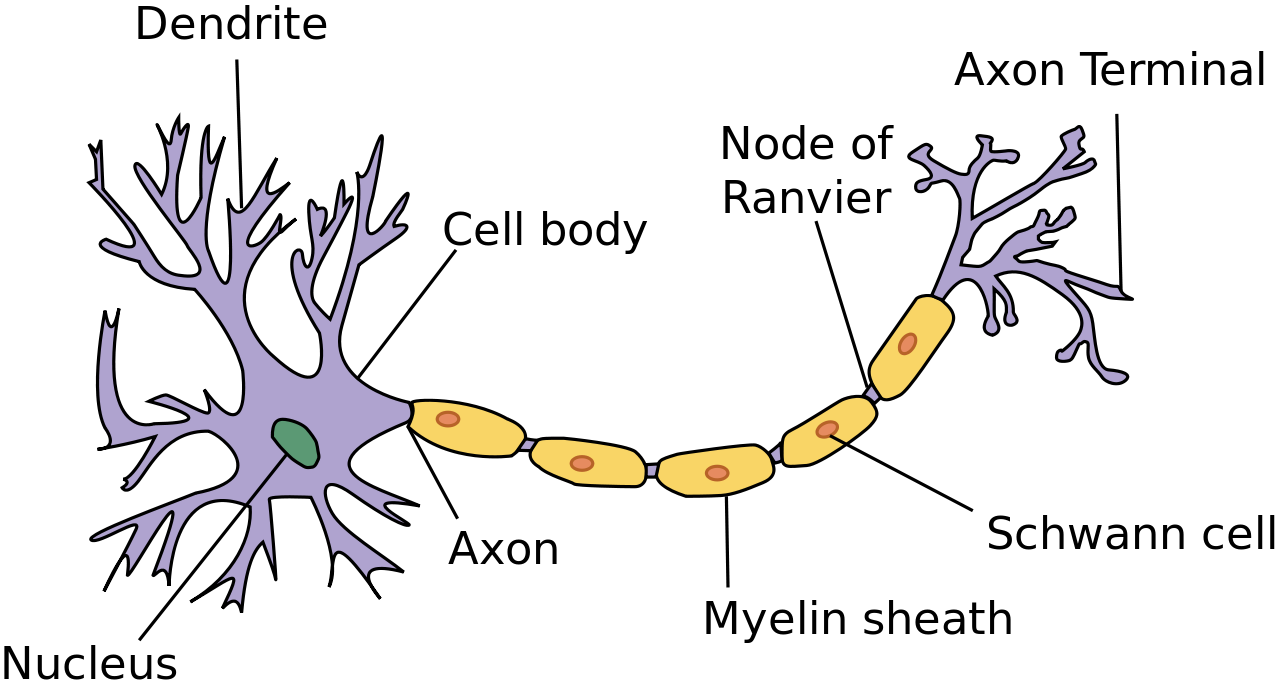
\includegraphics[scale=0.18]{charts/neuron.png}
		\caption{Ảnh neuron sinh học.\cite{img-neuron}}
		\label{fig:neuron}
	\end{figure}
	Mạng neural có gồm nhiều đơn vị kết nối, làm việc như một thể thống nhất thông qua việc trao đổi thông tin nhờ các liên kết.
	
	\subsection{Cấu trúc mạng neural}
	Như đã trình bày, các neuron trong một mạng làm việc như một thể thống nhất bằng việc trao đổi thông tin. Thực tế, đây là quá trình điều chỉnh các trọng số được truyền từ input ban đầu kết hợp với các hàm tính toán để có được các thông số trọng số phù hợp nhất. Quá trình này còn được gọi là quá trình học hay huấn luyện. Hình \ref{fig:NN} mô tả cấu trúc đơn giản nhất của một mạng neuron.
	\begin{figure}[h!]
		\centering
		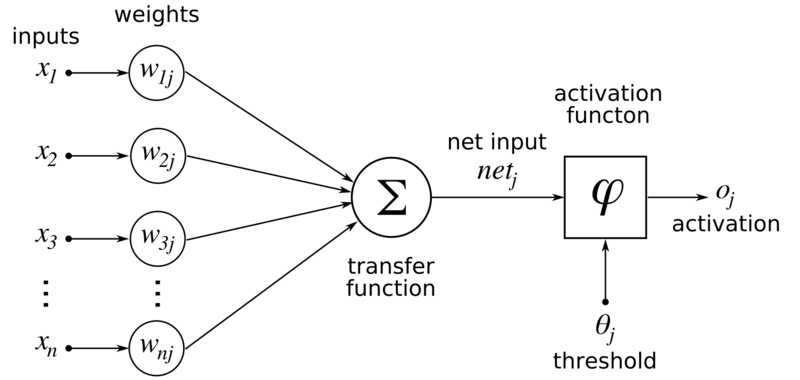
\includegraphics[scale=0.4]{charts/NN.png}
		\caption{Cấu trúc cơ bản mạng neuron.\cite{img-perceptron}}
		\label{fig:NN}
	\end{figure}
	\textbf{Cấu trúc mạng neuron\i}
	
	\begin{itemize}
		\item \textbf{Tập các node:} bao gồm nhiều node, mỗi node là đơn vị nhỏ nhất giữ chức năng xử lý thông tin của mạng.
		\item \textbf{Các tầng:} Các node trên được xếp thành các tầng, các node chung một tầng không thể kết nối nhau. Trong đó tầng input và tầng output là 2 tầng thiết yếu. Tùy vào một số mạng cụ thể có thể có thêm một hay nhiêu tầng nằm ở giữa được gọi là tầng ẩn (hidden layer).
		\begin{itemize}
			\item \textbf{\textit{Tầng input - input layer: }}các nối ở tầng này nhận dữ liệu đầu vào và truyền tới các node ở các tầng kế tiếp, trong một số trường hợp còn có chức năng xử lý thông tin.
			\item \textbf{\textit{Tầng ẩn - hidden layer: }}một số mạng có thể có thêm tầng ẩn, số lượng tầng ẩn trong một mạng có thể nhiều hơn 1. Có chức năng nhận các giá trị từ từng input hoặc tầng ẩn trước nó, tính toán các giá trị và gửi đến các node ở các tầng ẩn hoặc tầng ouput tiếp theo đó tùy theo từng mạng cụ thể.
			\item \textbf{\textit{Tầng output - output layer: }}nhận giá trị từ tầng trước đó (tầng ẩn hoặc tầng input) để tính toán các giá trị ngõ ra.
		\end{itemize}
		\item \textbf{Các liên kết:} mỗi node trong một tầng truyền thông tin qua các node ở các tầng khác thông qua các liên kết. Các giá trị mà các liên kết này được gán sẽ được gọi là trọng số liên kết (weight). Giá trị trọng số được kết nối vào neuron j với neoron k là \(w_{kj}\).
		\item \textbf{Hàm truyền - transfer function: }dùng để tính tổng các tích input với trọng số liên kết của nó. \[ \sum input_j*w_{ij}\]
		
		\item \textbf{Activation function: }dùng để tính toán giá trị input sang giá trị ouput. Tùy vào mục đích và cụ thể từng loại mạng mà có nhiều loại activation function khác nhau.\\
		Trong các bài toán khác nhau, người có những loại hàm activation như sau.
		
		\begin{itemize}
			\item \textbf{\textit{Step function: }} 
			\[ 
			\left \{
  			\begin{tabular}{cc}
  				0 & x < 0\\
  				1 &  x > 0 
  			\end{tabular}
		\right.
		\]
		\begin{figure}[h!]
			\centering
			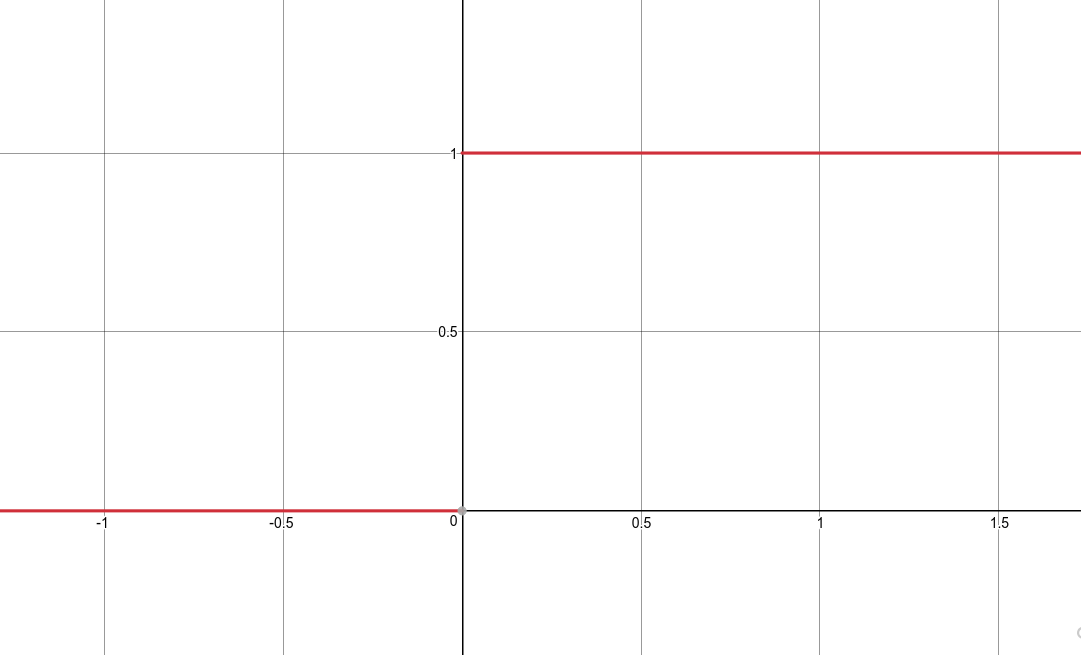
\includegraphics[scale=0.2]{charts/step_fun.png}
			\caption{Đồ thị hàm step}
			\label{fig:plot_step}
		\end{figure}
		
			\item \textbf{\textit{sigmoid function: }}
			\[A(x) =  \frac{1}{1 + e^{-x}}	\]
			\begin{figure}[h!]
				\centering
				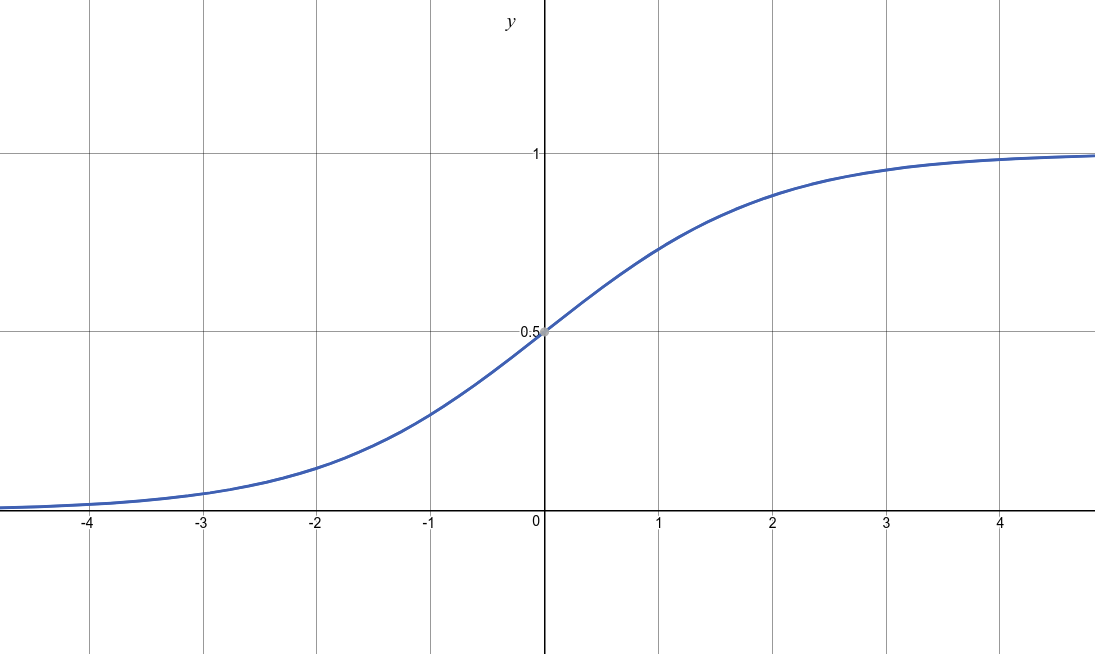
\includegraphics[scale=0.2]{charts/sigmoid_fun.png}
				\caption{Đồ thị hàm sigmoid}
				\label{fig:plot_sigmoid}
			\end{figure}
			\pagebreak
			
			\item \textbf{\textit{Tanh function:}}
			\[Tanh(x) = \frac{2}{1 + e^{-2x}} - 1 \]
			\begin{figure}[h!]
				\centering
				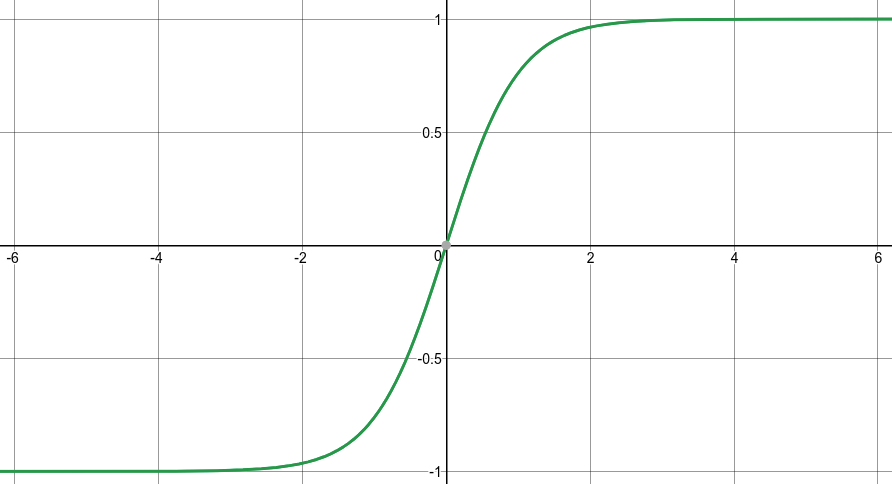
\includegraphics[scale=0.2]{charts/tanh_fun.png}
				\caption{Đồ thị hàm Tanh}
				\label{fig:plot_tanh}			
			\end{figure}
			
		\end{itemize}
		
	\end{itemize}
	
	\subsection{Mô hình Feedforward Neural Network}
	
		Thời điểm hiện nay, chúng ta có rất nhiều loại mô hình mạng neuron do sự khác nhau về sự kết hợp cũng như về mặt kiến trúc và thuật toán mà mạng đó áp dụng. Trong phần này, chúng ta sẽ tìm hiểu về mô hình mạng Feedforward Neural Network (FFNN), đây là kiến trúc mạng neuron được sử dụng phổ biến trong các bài toán dự báo. Mô hình gồm hai thành phần chính đó là kiến trúc feedforward - mạng truyền thẳng và giải thuật Backpropogation được áp dụng trong mạng.
		\subsubsection{Kiến trúc Feedforward}
			Đối với mạng feedfroward, cấu trúc gồm một tầng input, một tầng output và có thể có nhiều hơn một tầng ẩn nằm giữa hai tầng input và output. \\
			\begin{figure}[h!]
				\centering
				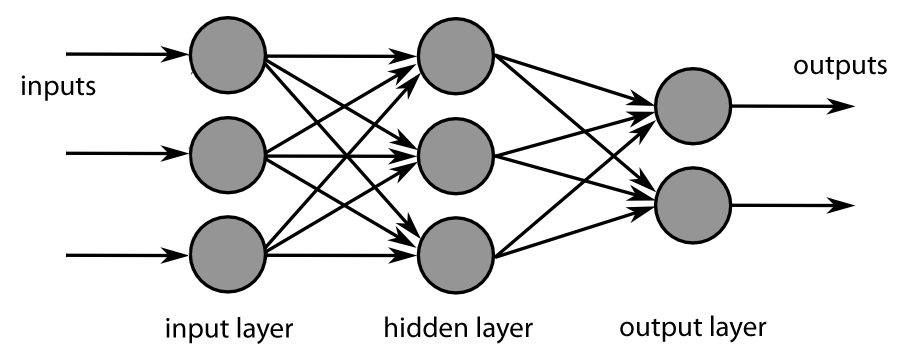
\includegraphics[scale=0.3]{charts/ffnn.png}
				\caption{Ví dụ kiến trúc mạng feeddorward}
				\label{fig:ffnn}			
			\end{figure}\\
			Như hình \ref{fig:ffnn}, một mạng Feedorward, trong tầng input và ouput thì số lượng neuron tại mỗi hai tầng nãy sẽ là cố định tùy theo đặc tính của dữ liệu. Đối với tầng ẩn, số lượng tầng ẩn cũng như số lượng neuron trong mỗi tầng tùy thuộc vào cá nhân thiết kế.
			
		\subsubsection{Giải thuật Backpropogation}
		Ở nội dung này, chúng ta sẽ không đi sâu vào kỹ thuật xử lý các phép tính\cite{dl} đạo hàm mà chỉ trình bày giải thuật lan truyền ngược một cách đơn giản nhất.\par
		Các ký hiệu và hàm được dùng trong trình bày giải thuật:
		\begin{itemize}
			\item \(W_{ij}\): là trọng số nối node thứ i tới node j ở layer kế tiếp.
			\item \(I_{j}\): là đầu vào tại node thứ j.
			\item \(O_{j}\): là kết quả xuất tại node thứ j.
			\item \(\theta_{j}\): bias tại node j.
			\item \(l\): tốc độ học của mạng (learning rate).
			\item \(Err_{j}\): giá trị lỗi tại node thứ j.
			\item Activation function được dùng trong nội dung này là hàm Sigmoid như mục trên
		\end{itemize}
		
		\begin{figure}[h!]
			\centering
			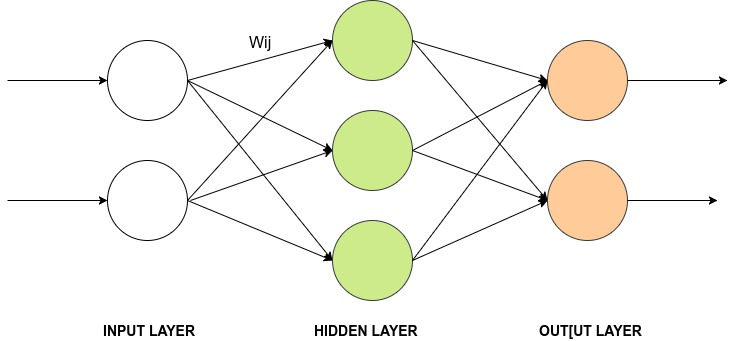
\includegraphics[scale=0.5]{charts/back.jpg}
			\caption{MLP}
			\label{fig:back}
		\end{figure}
		\pagebreak
		Nội dung thuật toán.\par
		\textbf{Input:}
		\begin{itemize}
			\item Mạng feed forward với n input, m node ở tầng ẩn, và p output.
			\item Hệ số học hay tốc độ học \(l\).
			\item Tập dữ hiệu huấn luyện \(D\).
			\item Sai số học \(\epsilon\).
		\end{itemize}
		\textbf{Output:} Vector các trọng số mới sau khi huấn luyện.
		
		\textbf{Nội dung thuật toán:}
		
		\begin{itemize}
			\item \textbf{Bước 1:} Khởi tạo ngẫu nhiên các giá trị trọng số  \(W_{ij}\).
			\item \textbf{Bước 2:} Tính toán các giá trị đầu vào \(I_{j}\) và đầu ra \(O_{j}\).
			\begin{itemize}
				\item Tại node i ở tầng input:
				\[I_{i} = x_{i}, O{i} = I_{i}\]
				\item Tại node j ở tầng khác:
				\[ I_{j} = \sum_{i} W_{ij}O_{i} + \theta_{j} \]
				\[O_{j} = \frac{1}{1 + e^{-I_{j}}}\]
			\end{itemize}
			\item \textbf{Bước 3:} Tính toán lỗi trung bình và đánh giá.
				\begin{itemize}
					\item Tại node thuộc tầng output:
					\[Err_{j} = O_{j}(1-O_{j})(T_{j} - O_{j})\]
					\item Tại node thuộc tầng ẩn:
					\[Err_{j} = O_{j}(1-O_{j})\sum_{k}Err_{k}W_{jk}\]
					Với \(Err_{k}, W_{jk}\) là giá trị lỗi tại node k ở tầng tiếp theo và giá trị trọng số của node j đến k.\\
					Thuật toán sẽ dừng lại khi \(Err_{k} \leq \epsilon\)
					
				\end{itemize}
			\item \textbf{Bước 4:} Cập nhật các trọng số và độ lệch
			\[W_{ij} = W_{ij} + (l)Err_{j}O_{i}\]
			\[\theta_{j} = \theta_{j} + (l)Err_{j}\]
			
			Thuật toán sẽ tiếp tục lặp lại bước 2 cho đến khi thỏa điều kiện dừng và cho ra các tập trọng số và độ lệch tốt nhất.
		\end{itemize}
	
			
			

\section{Mạng neural tích chập}

\subsection{Giới thiệu mạng neural tích chập}
	Trong vài năm trở lại đây, chúng ta thấy được sự nở rộ của các hệ thống thông minh từ các công ty công nghệ lớn trên thế giới. Các chức năng nhận dạng, phân loại hay dự đoán được áp dụng rộng rãi vào các lĩnh vực thương mại, vận tải..v..v.\par
	Mô hình Deep learning được sử dụng phổ biến và phát triển giúp các hệ thống thông minh có độ chính xác cao ngày nay chính là Convolutional Neural Networks(CNN) - mạng neuron tích chập. Trong các nội dung tới, chúng ta sẽ tìm hiểu các khái niệm, kiến trúc, cũng như ứng dụng của CNN trong lĩnh vực phân loại ảnh.

\subsection{Mô hình mạng neural tích chập}
	\subsubsection{Input và output}
		Phân loại ảnh là công đoạn chuyển hóa từ một đầu là một hình ảnh và kết quả là một nhãn ứng với hình ảnh đó hoặc là các xác suất mà hệ thống dự đoán dựa trên đặc điểm của ảnh. Với con người, công việc nhận diện này được hình thành từ khi mới sinh ra, chúng ta có thể đưa ra kết quả của một hình ảnh bất kỳ mà không chút khó khăn. Nhưng máy tính thì không đơn giản như vậy, đầu vào và kết quả phải được đưa về dạng kỹ thuật số mà máy có thể hiểu được.\par
		Khi một máy tính nhận vào một ảnh, nó sẽ thấy một mảng các giá trị pixel tùy thuộc vào kích thước và độ phân giải của ảnh\cite{overview}. Ví dụ, một ảnh màu có kích thước 224 x 224 pixel thì máy tính sẽ thấy hình ảnh này dưới dạng một mảng có kích thước 224 x 224 x 3, giá trị 3 do thuộc tính ảnh màu(RGB) mà có được, giá trị này sẽ là 1 nếu đây là ảnh trắng đen.\par
		Đối với ouput, đây là một mảng các giá trị xác suất, mảng giá trị này cũng tùy thuộc vào số lượng nhãn(lớp) cần dự đoán. Ví dụ, (0.90 cho xe ô tô, 0.1 cho xe tải).
	\subsubsection{Convolutional layer}
		Tầng đầu tiên của một mạng CNN luôn luôn là tầng tích chập (convolutional layer)\cite{conv}. Như đã biết đầu vào (input) là một mảng các giá trị pixel. Trong trường hợp cụ thể để dễ hình dung ta chọn input là mảng các giá trị pixel có kích thước 32 x 32 x 3 với 32 x 32 là chiều dài và chiều rộng của tấm hình và 3 là giá trị RGB khi là ảnh màu. Đối với input trên có nghĩa là sẽ có một ma trận có kích thước 32 x 32 pixel mỗi pixel sẽ chứa 3 giá trị mà mỗi giá trị đó lần lượt biểu diễn cho giá trị của 3 màu sắc trên máy tính là đỏ(RED), lục(GREEN) và làm(BLUE). \par
		Tạm thời bỏ qua giá trị RGB để đi vào cách hoạt động của tầng tích chập này. Cách đơn giản để giải thích cách hoạt động của tầng tích chập là tưởng tượng sẽ có một khuôn sẽ trượt từ phía trên bên trái cho đến hết tấm ảnh\cite{arch}. Với kích thước ảnh là 32 x 32 như trên, chọn kích thước ô trượt ví dụ là 5 x 5. Ô trượt có kích thước 5 x 5 sẽ trượt lần lượt qua cả input ảnh, ô trượt này được gọi là kernel hay filter(bộ lọc). Bộ lọc là một mảng các giá trị trọng số. Một điểm ghi chú là chiều sâu của bộ lọc sẽ bằng với chiều sâu của ảnh, với input 32 x 32 x 3 thì bộ lọc cũng sẽ có 5 x 5 x 3. Hình \ref{fig:conv_layer1} và \ref{fig:conv_layer2} minh họa cách kernel trượt trên input.
		%\pagebreak
		\begin{figure}[h!]
			\centering
			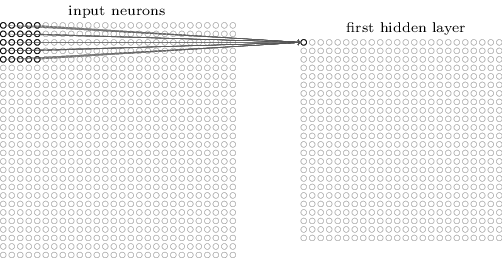
\includegraphics[scale=0.9]{charts/conv_layer1.png}
			\caption{Convolutional layer.\cite{conv-layer}}
			\label{fig:conv_layer1}
		\end{figure}
		
		\begin{figure}[h!]
			\centering
			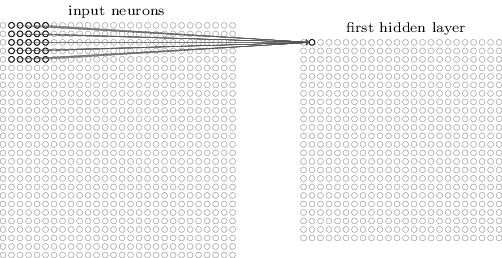
\includegraphics[scale=0.9]{charts/conv_layer2.png}
			\caption{Convolutional layer.\cite{conv-layer}}
			\label{fig:conv_layer2}
		\end{figure}
		
		Bây giờ ta sẽ đi vào việc mà tầng tích chập thực sự làm với những phép tính. Như đã trình bày rằng mỗi bộ lọc sẽ là một mảng các giá trị pixel, công dụng của mảng giá trị này nhằm mục đích phát hiện các đặc tính của mỗi vùng input mà filter trượt qua. Các đặc tính ở đây có thể là đường thẳng, đường cong, màu đơn giản. Ví dụ ta có một filter có kích thước là 7 x 7 x 3 dùng để phát hiện một dạng đường cong như hình \ref{fig:filter}.
		
		\begin{figure}[h!]
			\centering
			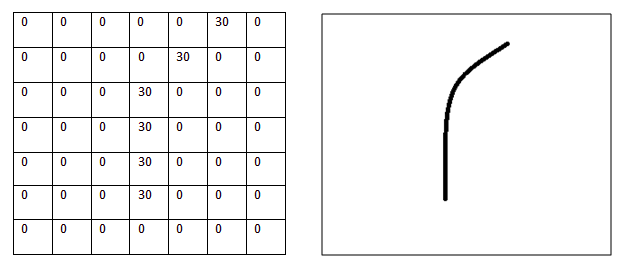
\includegraphics[scale=0.5]{charts/filter.png}
			\caption{Mảng các giá trị của bộ lọc \cite{conv-layer}}
			\label{fig:filter}
		\end{figure}
		
		Khi bộ lọc trên trượt đến vùng được đánh dấu vàng có dạng đường cong giống với bộ lọc như hình \ref{fig:mouse}. Lúc đó phép toán   tích châp sẽ được thực hiện như hình \ref{fig:conv_1} với ma trận bên trái chính là giá trị pixel của vùng được đánh dấu trên ảnh mà bộ lọc trượt tới, ma trận bên phải chính là bộ lọc được sử dụng hiện tại.
		
		\begin{figure}[h!]
			\centering
			
\includegraphics[scale=0.5]{charts/mouse.png}
			\caption{ảnh đầu vào \cite{img-input}}
			\label{fig:mouse}
		\end{figure}
		
		\begin{figure}[h!]
			\centering
			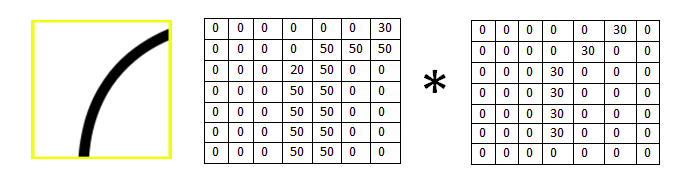
\includegraphics[scale=0.5]{charts/conv_1.png}
			\caption{phép toán tích chập \cite{img-input}}
			\label{fig:conv_1}
		\end{figure}
		
		Kết quả của phép tính trên sẽ có kết quả như sau:
		\[(50*30)+(50*30)+(50*30)+(20*30)+(50*30) = 6600 \]\\
	
		Đây là một con số rất lớn, thông thường nếu bộ lọc trượt tới một vùng mà vùng đó có hình dạng tương tự như bộ lọc thì kết quả khi thực hiện phép tính là một con số rất lớn. Ngược lại, kết quả sẽ ra rất nhỏ hoặc bằng 0. Ví dụ là hình ảnh \ref{fig:conv_2} kết quả sẽ là 0 khi thực hiện phép tính
		\begin{figure}[h!]
			\centering
			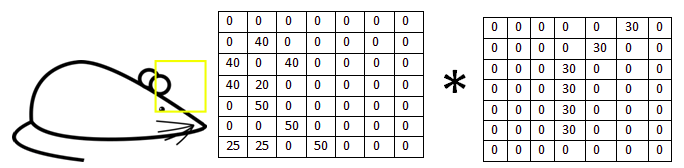
\includegraphics[scale=0.5]{charts/conv_2.png}
			\caption{phép toán tích chập \cite{img-input}}
			\label{fig:conv_2}
		\end{figure}
		
		Trên đây là mô tả đơn giản về tầng tích chập, trên thực tế, chúng ta có thể có nhiều bộ lọc để phát hiện các khuôn mẫu, hình dạng khác nhau trong ảnh đầu vào. Kết quả xuất của tầng tích chập thứ nhất còn được gọi là bản đồ đặc tính (feature map) và có thể có nhiều feature map cho một input sau khi hoàn thành tầng tích chập. Như \ref{fig:feature_map} biểu diễn một input kích thước như hình sau khi qua tầng tích chập và sử dụng tập các bộ lọc 5 x 5 cho ra tập 3 feature map mà mỗi cái nhận diện được một khuôn dạng khác nhau xuất hiện trong input.
		%\pagebreak
		\begin{figure}[h!]
			\centering
			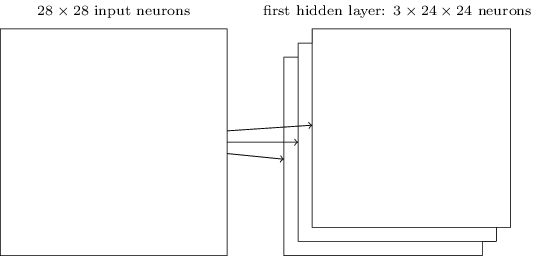
\includegraphics[scale=0.5]{charts/feature_map.png}
			\caption{kết quả tầng tích chập \cite{img-input}}
			\label{fig:feature_map}
		\end{figure}
	
	\subsubsection{Pooling Layer}		
		Sau khi qua một hoặc vài tầng tích chập, CNN sẽ chứa các tầng tổng hợp (Pooling Layer) ngay sau đó. Ở đây, tầng tổng hợp sẽ đơn giản hóa thông tin được lấy từ đầu ra từ tầng tích chập trước đó. Có nhiều kiểu tổng hợp khác nhau đối với tầng này, nhưng max-pooling là phép tổng hợp phổ biến được sử dụng. Hình \ref{fig:max-pooling} biểu diển một ví dụ phép max-pooling với một bộ lọc có kích thước là 2 x 2. Giá trị lớn nhất trong mỗi vùng được trượt qua sẽ được chọn làm kết quả xuất ra.
		
		\begin{figure}[h!]
			\centering
			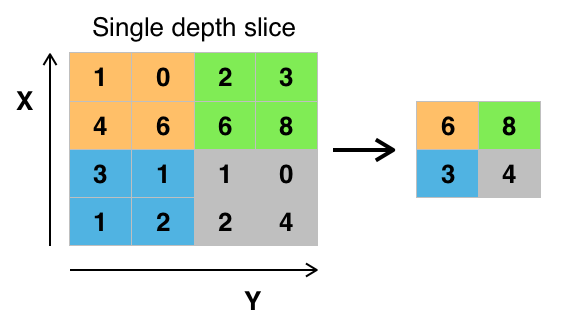
\includegraphics[scale=0.7]{charts/max_pooling.png}
			\caption{max-pooling 2 x 2 \cite{img-pool}}
			\label{fig:max-pooling}
		\end{figure}
		\pagebreak
		
		Công dụng của phép pooling này giúp giảm đi kích thước của tập miêu tả đặc trưng từ đó cũng làm cho số lượng tham số và tính toán giảm theo. Và do chúng ta có thể có nhiều feature map từ tầng tích chập nên phép tổng hợp cũng sẽ được áp dụng độc lập cho mỗi feature map. Nếu có 3 feature map thì sẽ có 3 phép tổng hợp trong trường hợp này là max-pooling.
		
		\begin{figure}[h!]
			\centering
			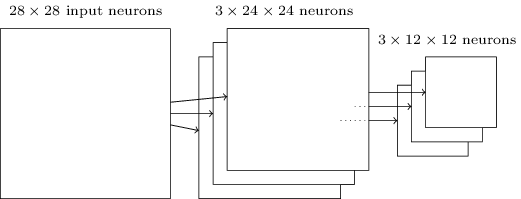
\includegraphics[scale=0.5]{charts/pooling_ex.png}
			\caption{Ví dụ tầng tổng hợp \cite{conv-layer}}
			\label{fig:pooling_ex}
		\end{figure}
		
	
	\subsubsection{Fully Connected Layer}
		Sau khi thông tin input đã qua các tầng tích chập và tổng hợp, các giá trị dữ liệu sẽ đi đến tầng fully connected để xuất ra kết quả. Kết quả tại tầng fully connected là một vector có kích thước bằng với số lớp(nhãn) mà bài toán cần dự đoán. Như bài toán phân loại ảnh giao thông ùn tắt và thông thoáng thì lúc này số nhãn cần dự đoán và kích thước vector tại tầng này sẽ bằng 2. Giá trị của các phần tử trong vector sẽ là giá trị xác suất của mỗi nhãn mà mạng dự đoán, [ 0.8, 0.2 ] sẽ biểu diễn 80\% ảnh này thuộc lớp 1 và 20\% ảnh thuộc lớp thứ 2. Về cơ bản, cách kết nối ở tầng này giống như cách kết nối neuron giữa các tầng với nhau ở mạng neuron ở mục trước. Khi đó, tất cả neuron ở tầng pooling sẽ kết nối với từng neuron trong tầng cuối.


\section{Tổng quan về hệ thống Apache Hadoop}
Apache Hadoop là một dự án phát triển phần mềm nhằm cung cấp một nền tảng phân tán, có thể mở rộng linh hoạt và có độ tin cậy cao.\par
Ngoài ra Hadoop còn được xem là một thư viện hay framework cho phép xử lý phân tán khối lượng lớn dữ liệu trên nhiều cụm máy tính bằng các mô hình lập trình. Framework nay được thiết kế với mục đích có khả năng mở rộng từ một máy chủ đơn lẻ lên đến rất nhiều trạm làm việc mà mỗi máy trạm có khả năng tính toán và lưu trữ cục bộ.
\section{Hadoop distributed file system - HDFS}
\subsection{Thiết kế}
HDFS là một hệ thống file nhằm lưu trữ một lượng rất rất lớn (Lớn ở đây theo nghĩa có thể là hàng trăm megabytes, gigabytes, hoặc terabytes) với cơ chế streamming data access trên những thiết bị phổ thông \footnote{các máy tính hoặc máy trạm}.
 Đây là cơ chế phân luồng dữ liệu trong HDFS với mục đích ghi một lần chạy nhiều lần. Điển hình là dữ liệu sẽ được sinh và sao chép từ nguồn và sau đó có rất nhiều tiến trình phân tích khác nhau thực thi dữ liệu trên. Mỗi hoạt động phân tích sẽ thực thi liên quan đến một phần nào đó khác nhau trên cả một tập dữ liệu trên.\par
 Từ các thiết bị phổ thông ở đây là những những thiết bị phần cứng máy tính, HDFS không yêu cầu một phần cứng đắt tiền hay độ tin cậy cao. Mà nó được thiết kế để chạy trên những cụm máy tính từ nhiều nhà cung ứng khác nhau. Vì thế mà xác suất để một node(đơn vị phần cứng) gặp lỗi và thất bại là rất lớn, đặc biệt là những cụm có hàng ngàn máy trạm. Với đặc tính đó, HDFS được thiết kế sao cho không có sự gián đoạn nào được phát hiện ở người dùng khi mà việc một số lượng node gặp lỗi giữa chừng.\par
\subsection{Các khái niệm trong HDFS}
\begin{itemize}
	\item \textbf{Block(sector): }trong các đĩa cứng thông thường, đây là các phần nhỏ cuối cùng được chia ra để chứa dữ liệu, và đây cũng là đơn vị nhỏ nhất mà một lần đọc và ghi dữ liệu được hiện thực. Thông thường, block ở các đĩa cứng có dung lượng nhỏ chỉ tầm 512 byte. Ở HDFS, block thường có dung lượng lớn hơn rất nhiều - mặc định là 128MB. Do dung lượng của một block trên đĩa lớn như vậy nên các file tập tin trong HDFS nhiều khi có dung lượng và được lưu trữ nằm trong cả một block (trong HDFS). Nguyên nhân của việc block trong HDFS có dung lượng lớn như vậy là nhằm việc tối thiểu hóa chi phí tìm kiếm \cite{hadoop-def}
	\item \textbf{Namenodes và Datanodes: }một HDFS gồm nhiều node, trong đó có hai loại chính đó là một master node (Namenode) - máy chủ và nhiều datanodes (những thiết bị nô lệ). Namenode là chương trình chỉ đạo các datanodes thực hiện các nhiệm vụ I/O ở mức thấp. Còn datanodes được sự điều phối của Namenode, lưu trữ và thường xuyên báo cáo với master các khối(block) mà nó hiện đang lưu trữ. Ngoài ra, các datanodes còn giao tiếp với nhau để sao lưu các khối dữ liệu dự phòng.
	\item \textbf{jobTracker: }Trình nền JobTracker là một liên lạc giữa ứng dụng của bạn và Hadoop. Một khi bạn gửi mã nguồn của bạn tới các cụm (cluster), JobTracker sẽ quyết định kế hoạch thực hiện bằng cách xác định những tập tin nào sẽ xử lý, các nút được giao các nhiệm vụ khác nhau, và theo dõi tất cả các nhiệm vụ khi chúng đang chạy. Nếu một nhiệm vụ (task) thất bại (fail), JobTracker sẽ tự động chạy lại nhiệm vụ đó, có thể trên một node khác, cho đến một giới hạn nào đó được định sẵn của việc thử lại này.
Chỉ có một JobTracker trên một cụm Hadoop. Nó thường chạy trên một máy chủ như là một nút master của cluster.
\item \textbf{TaskTraker: }Như với các trình nền lưu trữ, các trình nền tính toán cũng phải tuân theo kiến trúc master/slave: JobTracker là giám sát tổng việc thực hiện chung của một công việc MapRecude và các taskTracker quản lý việc thực hiện các nhiệm vụ riêng trên mỗi node slave.
Mỗi TaskTracker chịu trách nhiệm thực hiện các task riêng mà các JobTracker giao cho. Mặc dù có một TaskTracker duy nhất cho một node slave, mỗi TaskTracker có thể sinh ra nhiều JVM để xử lý các nhiệm vụ Map hoặc Reduce song song. Một trong những trách nhiệm của các TaskTracker là liên tục liên lạc với JobTracker. Nếu JobTracker không nhận được nhịp đập từ một TaskTracker trong vòng một lượng thời gian đã quy định, nó sẽ cho rằng TaskTracker đã bị treo (cashed) và sẽ gửi lại nhiệm vụ tương ứng cho các nút khác trong cluster.Cấu trúc liên kết này có một node Master là trình nền NameNode và JobTracker và một node đơn với SNN trong trường hợp node Master bị lỗi. Đối với các cụm nhở, thì SNN có thể thường chú trong một node slave. Mặt khác, đối với các cụm lớn, phân tách NameNode và JobTracker thành hai máy riêng. Các máy slave, mỗi máy chỉ lưu trữ một DataNode và Tasktracker, để chạy các nhiệm vụ trên cùng một node nơi lưu dữ liệu của chúng
\end{itemize}
\subsection{HIVE}
Hive là hạ tầng kho dữ liệu cho Hadoop. Nhiệm vụ chính là cung cấp sự tổng hợp dữ liệu, truy vấn và phân tích. Nó hỗ trợ phân tích các tập dữ liệu lớn được lưu trong HDFS của Hadoop cũng như trên Amazon S3. Điểm hay của HIVE là hỗ trợ truy xuất giống SQL đến dữ liệu có cấu trúc, được biết với tên HiveSQL (hoặc HQL) cũng như phân tích big data với MapReduce. Hive không được xây dựng để hồi đáp nhanh các câu truy vấn nhưng nó được xây dựng cho các ứng dụng khai thác dữ liệu (data mining). Các ứng dụng khai thác dữ liệu có thể mất nhiều phút đến nhiều giờ để phân tích dữ liệu và HIVE được dùng chủ yếu.\par 
\subsubsection{Cách tổ chức của HIVE}
Dữ liệu được tổ chức thành 3 định dạng trong HIVE.\par

\textbf{Tables:} Chúng rất tương tự như bảng (tables) trong RDBMS và chứa các dòng (rows). Hive chỉ được xếp lớp trên HDFS, do đó tables được ánh xạ trực tiếp vào các thư mục của hệ thống tập tin. Nó cũng hỗ trợ các tables được lưu trên các hệ thống tập tin khác.\par

\textbf{Partitions:} Hive tables có thể có nhiều hơn 1 partition. Chúng được ánh xạ với các thư mục con và các hệ thống tập tin.\par

\textbf{Buckets:} Trong Hive, dữ liệu có thể được chia thành các buckets. Buckets được lưu trữ như các tập tin trong partition trong hệ thống tập tin.\par
Hive cũng có metastore để lưu tất cả metadata. Nó là cơ sở dữ liệu quan hệ chứa thông tin khác nhau liên quan đến Hive Schema (column types, owners, key-value data, statistics,…). Chúng ta có thể dùng MySQL cho việc này.
\subsubsection{HIVESQL}
Ngôn ngữ truy vấn Hive cung cấp các toán tử cơ bản giống SQL. Đây là một số tác vụ mà HQL có thể làm dễ dàng.
\begin{itemize}
	\item Tạo và quản lý tables và partitions.
	\item Hỗ trợ các toán tử Relational, Arithmetic và Logical khác nhau.
	\item Evaluate functions
	\item Tải về nội dung 1 table từ thư mục cục bộ hoặc kết quả của câu truy vấn đến thư mục HDFS.
	\item Đây là ví dụ truy vấn HQL:
	\begin{lstlisting}[language=SQL]
SELECT upper(name), salesprice 
FROM sales; 
SELECT category, count(1) 
FROM products 
GROUP BY category;

	\end{lstlisting}
\end{itemize}
\section{ Tại sao sử dụng Apache Hadoop trong đề tài}
Hiện nay trên các xe buýt đều được trang bị camera hành trình, các video này ghi lại hình ảnh trên các con đường. Các hình ảnh này được gửi về hệ thống một cách liên tục hàng ngày và hàng giờ. Do kích thước dữ liệu tăng lên đáng kể cần một hệ thống lưu trữ có khả năng mở rộng linh động, vì thế hệ thống HDFS do Apache Hadoop hỗ trợ là công cụ hợp lý. Ngoài ra hệ thống HDFS còn có thể kết hợp với các thư viện hỗ trợ học sâu như Tensorflow nên ta có thể áp dụng các mô hình trong lĩnh vực machine learning nói chung và deep learning nói riêng để xây dựng một hệ thống phân loại ảnh. Khi kết hợp các thành phần trên, ta có thể tinh chỉnh tập dữ liệu sao cho phù hợp với bài toán của thể của từng trường hợp cũng như các lĩnh vực khác mà không nhất thiết là lĩnh vực giao thông.

	
	
	
	
